\chapter{Problemas de Optimización de Diseño de Mecatrónico} 
\label{Chapter5} 
En el capítulo introductorio del presente trabajo se abordaron algunos conceptos fundamentales sobre el Diseño Mecatrónico:
\begin{enumerate}
\item El modelado de un sistema mecatrónico tiene como objetivo representar el comportamiento de un sistema real mediante un conjunto de ecuaciones matemáticas.
\item Los sistemas reales son sistemas físicos, cuyo comportamiento se basa en la materia y la energía.
\item   Los modelos utilizados en el diseño mecatrónico representan estructuras de causa y efecto, aceptan información externa y la procesan con su lógica y ecuaciones para producir una o más salidas. 
\item El objetivo de la optimización es, dado un modelo de un sistema determinado físico, encontrar una configuración óptima para este sistema. 
\end{enumerate}
Estos conceptos son la base para el desarrollo de la siguientes secciones. En adelante se describen primeramente tres casos de estudio de la "Síntesis Óptima de un Mecanismo de Cuatro Barras", luego se presentan dos casos de la "{Síntesis Óptima de un Efector Final de Tres Dedos}". Por último, se presenta el problema de "{Optimización del costo de generación de energía en una Micro-red Eléctrica no Interconectable}". Estos problemas han sido formulados y resueltos por investigadores del departamento de mecatrónica del Centro de Innovación y Desarrollo Tecnológico en Cómputo (CIDETEC) del Instituto Politécnico Nacional (IPN), lo que brinda un marco de referencia tanto desde el punto de vista del problema (conocimiento de óptimos) como en el conocimiento del desempeño de los algoritmos utilizados (número de evaluaciones, rapidez de convergencia, resultados de pruebas estadísticas).
\section{Diseño cinemático de Mecanismos}\label{sec: Diseño cinemático de Mecanismos}
Las máquinas son dispositivos utilizados para alterar, transmitir y dirigir las fuerzas para lograr un objetivo específico. Un mecanismo es la parte mecánica de una máquina que tiene la función de transferir movimiento y fuerzas desde una fuente de alimentación a una salida. Los mecanismos se pueden considerar como piezas rígidas que están dispuestas y conectadas para que produzcan el movimiento deseado de la máquina. Los mecanismos de enlace son aquellos compuestos por diferentes eslabones (barras) conectados entre sí para formar una cadena. Los eslabones son las partes individuales del mecanismo y se consideran cuerpos rígidos que se encadenan  para transmitir movimiento y fuerza. Teóricamente, un cuerpo rígido no cambia de forma durante el movimiento. A pesar de que no existe un verdadero cuerpo rígido, pues los componentes del mecanismo siempre están sujetos a ciertas deformaciones, en lo adelante se consideran estos componentes como cuerpos rígidos, atendiendo solo al análisis cinemático. En los mecanismos de enlace un eslabón se designa como marco (frame en inglés) de referencia para el movimiento de todas las otras partes. El marco de referencia es típicamente un eslabón que no realiza movimiento. Entre dos eslabones existe una conexión movible que permite el movimiento relativo entre estos, llamada \textit{junta}. Las articulaciones básicas pueden ser clasificadas en giratorias y deslizantes. La articulación giratoria permite la rotación pura entre los dos enlaces que conecta. La junta deslizante también llamada pistón o junta prismática, permite el deslizamiento lineal entre los enlaces conectados. Además existen otros tipos de juntas como la junta de leva que permite tanto la rotación como el deslizamiento entre los dos enlaces que conecta. La junta de engranaje también permite la rotación y el deslizamiento entre dos engranajes. Ambos tipos de juntas son consideradas articulaciones de orden superior debido a que permiten movimientos más complejos \cite{myszka2004machines}.

La síntesis es el proceso de desarrollar un mecanismo para satisfacer un conjunto de requisitos de rendimiento para una máquina. De forma general, la cinemática estudia el movimiento de los cuerpos sólidos. Aplicada al diseño de mecanismos, se utiliza para analizar la geometría del movimiento, lo que implica el análisis de la posición, el desplazamiento, la rotación, la velocidad, y la aceleración de los componentes. Por tanto, el análisis cinemático asegura que el mecanismo mostrará un movimiento que cumplirá con determinado conjunto de requisitos. Para lograr la síntesis óptima de un mecanismo es necesario recurrir a técnicas analíticas avanzadas que implican el modelado mediante funciones matemáticas. Las técnicas analíticas combinan las teorías de geometría, trigonometría y análisis de mecanismos gráficos. La síntesis óptima comprende la modelación de estos mecanismos matemáticamente, en forma de problemas de optimización numérica. Estos problemas pueden ser resueltos mediante algunas de las técnicas abordadas en capítulos anteriores \cite{myszka2004machines}. 


\subsection{Análisis cinemático de un Mecanismo de Cuatro Barras}\label{sec:Análisis cinemático de un Mecanismo de Cuatro Barras}
El mecanismo de cuatro barras es una combinación de cuatro eslabones, que están conectado por cuatro juntas de giratorias. Este mecanismo tiene una gran cantidad de aplicaciones por lo que se encuentra frecuentemente en la literatura. 


El esquema general del mecanismo de cuatro barras que se muestra en la Figura \ref{fig:MEC}. Está formado por una barra de referencia $r_1$, una barra de entrada $r_2$ (manivela), un acoplador $r_3$ y una barra de salida $r_4$ (basculante). Para analizar este mecanismo se establecen dos sistemas de coordenadas: un sistema que se fija al mundo real ($OXY$) y otro para la auto-referencia \cite{herne1_two_swim_2016}.

\begin{figure}[htb]
    \centering
    \resizebox {\textwidth} {\height} {
     \includegraphics[width=0.6\textwidth]{MEC.tikz}
     }
    \caption{Mecanismo de cuatro barras.}
    \label{fig:MEC}
\end{figure}
Para el análisis de la posición, velocidad y aceleración se comienza por plantear las ecuaciones que describen el hecho de que las barras del mecanismo conforman un lazo cerrado:

\begin{equation}\label{eq:MElazo}
\vec{r_1}+\vec{r_4}=\vec{r_2}+\vec{r_3}
\end{equation}
 En la Ecuación \ref{eq:MElazo} las barras son consideras vectores. Como cualquier vector puede ser expresado como un número complejo utilizando notación polar, donde la parte real corresponde al eje de las abscisas y la parte imaginaria pertenece al eje de las coordenadas. Luego, la Ecuación \ref{eq:MElazo} puede ser expresada en coordenadas polares de la siguiente forma:
\begin{equation}\label{eq:MElazoPolar}
r_1e^{j\theta_1}+r_4e^{j\theta_4}=r_2e^{j\theta_2}+r_3e^{j\theta_3}
\end{equation}
Donde $e^{j\theta_1}$ es la entidad de Euler y $\theta_i$ es el ángulo comprendido entre cada barra y el eje de coordenadas. La identidad de Euler plantea la siguiente relación donde $j$ es la unidad imaginaria \cite{weisstein_euler_nodate}:
\begin{equation}\label{eq:Euler}
 e^{jx}=\cos{x}+j\sin{x} 
\end{equation}


Luego sustituyendo la Ecuación \ref{eq:Euler} en \ref{eq:MElazoPolar} se obtiene la expresión:
\begin{equation}\label{eq:MEPolarEuler}
r_1(\cos{\theta_1}+j\sin{\theta_1})+r_4(\cos{\theta_4}+j\sin{\theta_1})=r_2(\cos{\theta_2}+j\sin{\theta_2})+r_3(\cos{\theta_3}+j\sin{\theta_3})
\end{equation}
Resolviendo:
\begin{equation}\label{eq:MEPolarEuler2}
r_1 \cos{\theta_1}+r_1 j \sin{\theta_1}+r_4\cos{\theta_4}+r_4j\sin{\theta_4}=r_2\cos{\theta_2}+r_2 j\sin{\theta_2}+r_3\cos{\theta_3}+r_3j\sin{\theta_3}
\end{equation}
Agrupando la real en el miembro izquierdo y la parte imaginaria en el miembro derecho:
\begin{equation}\label{eq:MEPolarEuler21}
r_1 \cos{\theta_1}+r_4\cos{\theta_4}- r_2\cos{\theta_2}-r_3\cos{\theta_3}=r_2 j\sin{\theta_2}+r_3j\sin{\theta_3} -r_1 j \sin{\theta_1}-r_4j\sin{\theta_4}
\end{equation} 
Separando la parte real y la parte imaginaria en un sistema de ecuaciones se obtiene:
\begin{eqnarray}
r_1 \cos{\theta_1}+r_4\cos{\theta_4}&=&r_2\cos{\theta_2} +r_3\cos{\theta_3} \label{eq:MEPolarEuler4} \\
r_1j\sin{\theta_1}+r_4j\sin{\theta_4} &=&r_2j\sin{\theta_2}+r_3j\sin{\theta_3}\label{eq:MEPolarEuler3}
\end{eqnarray}
Dividiendo por la unidad imaginaria en la ecuación \ref{eq:MEPolarEuler3}: 
\begin{eqnarray}
r_1 \cos{\theta_1}+r_4\cos{\theta_4}&=&r_2\cos{\theta_2} +r_3\cos{\theta_3} \label{eq:MEPolarEuler5} \\
r_1\sin{\theta_1}+r_4\sin{\theta_4} &=&r_2\sin{\theta_2}+r_3\sin{\theta_3}\label{eq:MEPolarEuler6}
\end{eqnarray}
Este sistema de ecuaciones se expresa en función de $\theta_4$ para obtener:
\begin{eqnarray}
r_4\cos{\theta_4}&=&r_2\cos{\theta_2} +r_3\cos{\theta_3}-r_1 \cos{\theta_1}\label{eq:MEPolarEuler7} \\
r_4\sin{\theta_4} &=&r_2\sin{\theta_2}+r_3\sin{\theta_3}-r_1\sin{\theta_1}\label{eq:MEPolarEuler8}
\end{eqnarray}
Se obtiene la ecuación compacta de Freudenstein elevando al cuadrado y sumando los términos
del sistema de ecuaciones anterior:
\begin{equation} \label{eq:A1B1C1}
 A_1\cos{\theta_3}+B_1\sin{\theta_3}+C_1=0 
\end{equation}
Donde:
\begin{eqnarray}
A_1&=& 2r_3(r_2\cos{\theta_2}-r_1\cos{\theta_1}) \label{eq:A1} \\
B_1&=& 2r_3(r_2\sin{\theta_2}-r_1\sin{\theta_1}) \label{eq:B1} \\
C_1&=& r_1^2+r_2^2+r_3^2-r_4^2 -2r_1r_2\cos(\theta_1-\theta_2) \label{eq:C1}
\end{eqnarray}
El ángulo $\theta_3$ se puede obtener como función de $A_1$, $B_1$, $C_1$ y $\theta_2$, si $\sen{\theta_3}$ y $\cos{\theta_3}$  se expresan en términos de $\tan(\frac{\theta_3}{2})$:
\begin{eqnarray}
\sin{\theta_3}= \frac{2tan(\frac{\theta_3}{2})}{1+tan^2(\frac{\theta_3}{2})}&,& \cos{\theta_3}= \frac{1-tan^2(\frac{\theta_3}{2})}{1+tan^2(\frac{\theta_3}{2})} \label{eq:enFuncionTheta3}
\end{eqnarray}

Sustituyendo la Ecuación \ref{eq:enFuncionTheta3} en la Ecuación \ref{eq:A1B1C1} se obtiene una ecuación no lineal de segundo orden:
\begin{equation} \label{eq:Lineal2dOrden}
 \left[C_1 -A_1\right]= tan^2{\frac{\theta_3}{2}}+\left[2B_1\right]\tan{(\frac{\theta_3}{2})}+A_1+C1=0
\end{equation}
Resolviendo la ecuación \ref{eq:Lineal2dOrden} el ángulo $\theta_3$ puede ser expresado de la siguiente forma:
\begin{equation} \label{eq:Lineal2dOrden_resuelta}
\theta_3= 2\arctan \left[ \frac{-B_1 \pm \sqrt{B^2_1+A^2_1-C^2_1}}{C_1-A_1} \right]
\end{equation}
El ángulo $\theta_4$ se obtiene de forma similar, seleccionando el signo del radical para los
ángulos $\theta_3$ y $\theta_4$ se seleccionan de acuerdo a la configuración del mecanismo según
la Tabla \ref{tab:Signo del radical}.
\begin{table}[]
\centering
\begin{tabular}{|l|l|l|}
\hline
\textbf{Configuración}& $\theta_3$& $\theta_4$  \\ \hline
abierto &  $+ \sqrt{}$&   $- \sqrt{}$  \\ \hline
cerrado & $- \sqrt{}$ & $ + \sqrt{}$  \\ \hline
\end{tabular}
\caption{Signo del radical según el tipo de mecanismo.}
\label{tab:Signo del radical}
\end{table}

Debido a que el punto de interés del acoplador es $C$, se establece la siguiente ecuación para determinar su posición en el sistema $O_2 X_r Y_r$:

\begin{eqnarray}
C_{xr}&=&r_2\cos{\theta_2} +r_{cx}\cos{\theta_3}-r_{cy}\sin{\theta_3} \label{eq:Cxr} \\
C_{yr}&=&r_2\sin{\theta_2} +r_{cy}\sin{\theta_3}+r_{cy}\cos{\theta_3}\label{eq:Cyr}
\end{eqnarray}
En el sistema global de coordenadas, este punto puede expresarse como:
\begin{equation}
 \begin{bmatrix}
  C_x\\
  C_y
\end{bmatrix}=
 \begin{bmatrix}
  \cos{\theta_0} & -\sin{\theta_0} \\
    \sin{\theta_0} & \cos{\theta_0} 
\end{bmatrix}
 \begin{bmatrix}
  C_{xr}\\
  C_{xy}
\end{bmatrix}+
 \begin{bmatrix}
  x_0\\
  y_0
\end{bmatrix}
 \end{equation}
Las ecuaciones anteriores permiten calcular la trayectoria del punto $C$ durante el movimiento de  las barras del mecanismo. Teniendo en cuenta este análisis cinemático se puede encontrar una configuración para los componentes del mecanismo tal que el punto $C$ recorra una trayectoria deseada. 

\subsection{Planteamiento del Problema de Optimización para casos de estudio del Mecanismo de Cuatro Barras}
Con base en el análisis cinemático abordado en la Sección \ref{sec:Análisis cinemático de un Mecanismo de Cuatro Barras} se plantea un problema de optimización numérico que tiene como objetivo minimizar el error entre el punto $C$ del acoplador y ciertos puntos de precisión para describir una trayectoria determinada. Los componentes del mecanismo como las  barras y los ángulos de rotación están sujetas ciertas restricciones para garantizar el movimiento. 

\subsubsection{Función Objetivo}\label{sec:Funcion Objetivo de MEC}
La síntesis óptima del mecanismo de cuatro barras persigue hallar una configuración que permita la máxima precisión del mecanismo al realizar una trayectoria deseada. Esto significa que se deben encontrar las longitudes de las barras, el ángulo de rotación respecto al eje $OXY$, la distancia entre los dos sistemas de referencias, los valores para el conjunto de ángulos para la barra de entrada que permitirán generar la trayectoria deseada. Esta trayectoria puede ser lograda definiendo un conjunto de puntos de precisión. En el sistema global de coordenadas el punto de precisión $i$ esta dado por:
\begin{equation}
C^i_d=\left[C^i_x,C^i_y \right],
\end{equation}
El conjunto de los $N$ puntos se define entonces como:
\begin{equation}
\Omega=\left \{ C^i_d | i \in N \right \}
\end{equation}
Partiendo de las análisis cinemático descrito en la sección \ref{sec:Análisis cinemático de un Mecanismo de Cuatro Barras} se conoce que dado un conjunto de valores de las barras del mecanismo y sus parámetros $x_0$, $y_0$, $\theta_0$, la posición del acoplador puede ser expresada como una función de la posición de la barra de entrada: 
\begin{equation}
C^i=\left[C_x\left(\theta_2\right),C_y\left(\theta_2 \right) \right],
\end{equation}
Luego, para maximizar la precisión del mecanismo es necesario minimizar la distancia entre los puntos de precisión $C^i_d$ y los puntos calculados $C^i$. La función propuesta para dicho cálculo es:
\begin{equation}
f(\theta^i_2)= \sum_{i=1}^{N} \big[\big(C^{i}_{xd}-C^{i}_{x} \big)^2 +\big(C^{i}_{yd}-C^{i}_{y} \big)^2\big]
\end{equation}
\subsubsection{Restricciones de diseño}\label{sec:Restricciones de diseño MEC}
Las restricciones aplicadas al mecanismo de cuatro barras están dirigidas a garantizar la movilidad del mecanismo y a cumplir con especificaciones de dimensionamiento. las restricciones relacionadas con la movilidad del mecanismo se derivan de las \textit{Ley de Grashoff} las cuales establecen el tipo de movimiento del mecanismo de cuatro barras atendiendo a la longitud de sus elementos. Shigley define lo siguiente en \cite{shigley1983teoria}:
\begin{quote}
\textit{``{En un eslabonamiento plano de cuatro barras, la suma de las longitudes más corta y más larga de los eslabones no puede ser mayor que la suma de las longitudes de los dos eslabones restantes, sí se desea que exista una rotación relativa continua entre dos elementos}."} 
\end{quote}
Si se aplica la convención de que el eslabón más largo tiene la longitud $l$, la del más corto es $s$ y los otros dos tienen las longitudes $p$ y $q$. La ley de Grashof especifica que uno de los eslabones, en particular el más pequeño, podrá girar continuamente en relación con los otros tres sólo cuando se satisfaga la siguiente desigualdad:
\begin{equation}
s+l \leq p+q
\end{equation}
De forma análoga se platea la ley de Grashoff para el mecanismo de cuatro barras en cuestión:
\begin{equation}
r_1+r_2 \leq r_3+r_4
\end{equation}
Además de estas condiciones, se deben tomar en cuenta las siguientes restricciones  para asegurar que el mecanismo cumpla con la ley de Grashof:
\begin{equation}
r_2 < r_3;\quad r_3 < r_4;\quad r_4 < r_1 
\end{equation}
Debido a que el problema de la síntesis es de generación de trayectoria sin sincronizan prescrita, los valores que toman los ángulos de la manivela deben estar ordenados secuencialmente. Si el ángulo
del punto de precisión $i$ se denota como $\theta^i_2$ , se debe cumplir que:
\begin{equation}
\theta^1_2 < \theta^2_2< ... < \theta^N_2
\end{equation}
\subsection{Caso de estudio 1: seguimiento de una trayectoria lineal vertical, sin
sincronización previa - MCE1}
El presente caso de estudio es tomado de \cite{VegaMEC1}, en el cual el acoplador debe pasar por
seis puntos de precisión indicados en la Ecuación \ref{eq:Puntos de Presicion MEC1}, los cuales se encuentran alineados verticalmente.
\begin{equation}\label{eq:Puntos de Presicion MEC1}
\Omega = \left \{ (20, 20), (20, 25), (20, 30), (20, 35), (20, 40) (20, 45)\right\} 
\end{equation}
El vector de variables para este caso está constituido por 15 componentes:
\begin{eqnarray}\label{eq:Vector variables MEC1}
\vec{p} &=& \{p_1,p_2,p_3,...,p_{15} \}\\
       &=& \{ r_1,r_2,r_3,r_4,r_{cx},r_{cy},\theta_0,x_0,y_0,\theta_1,\theta_2,\theta_3,\theta_4,\theta_5,\theta_6 \} 
\end{eqnarray}
Las primeras cuatro variables en el vector de diseño corresponde a los valores de la longitud de las barras, las dos variables siguientes $r_{cx}$ y $r_{cy}$ describen la posición del acoplador, $\theta_0$, $x_0$ y $y_0$ indican la la posición del sistema de referencia $O_2X_rY_r$ con respecto al sistema $OXY$ , y las variables restantes corresponden a la secuencia de ángulos de la barra de entrada $r_2$.

Los límites superior e inferior de las variables de diseño se encuentran definidos
por:
\begin{eqnarray}\label{eq:limites variables MEC1}
r_1,r_2,r_3,r_4& \in & \left[ 0,60\right] \\
r_{cx},r_{cy},\theta_0,x_0,y_0 & \in & \left[ -60,60\right] \\
\theta_1,\theta_2,\theta_3,\theta_4,\theta_5,\theta_6& \in & \left[ 0,2\pi \right] \\
\end{eqnarray}
El problema de optimización mono-objetivo para el este caso de estudio se define como:
 \begin{equation}\label{}
 \begin{aligned}
min\quad  f(\vec{p})=
\sum_{i=1}^{N}\big[\big(C^{i}_{xd}-C^{i}_{x} \big)^2 +\big(C^{i}_{yd}-C^{i}_{y} \big)^2\big]
\\
\vec{p} \in  {\rm I\!R}^{15}
\\
\end{aligned}
\end{equation}
%1 () =  ⃗ 1 + 2 − 3 − 4 ≤ 0,
s.a:
\begin{eqnarray}\label{eq:Restricciones MEC1}
g_{1}(\vec{p})&=&p_{1}+ p_{2}-p_{3}-p_{4} \leq 0,\\
g_{2}(\vec{p})&=&p_{2}-p_{3} \leq 0,\\
g_{3}(\vec{p})&=&p_{3}-p_{4} \leq 0,\\
g_{4}(\vec{p})&=&p_{4}-p_{1} \leq 0,\\
g_{5}(\vec{p})&=&p_{10}-p_{11} \leq 0,\\
g_{6}(\vec{p})&=&p_{11}-p_{12} \leq 0,\\
g_{7}(\vec{p})&=&p_{12}-p_{13} \leq 0,\\
g_{8}(\vec{p})&=&p_{13}-p_{14} \leq 0,\\
g_{9}(\vec{p})&=&p_{14}-p_{15} \leq 0
\end{eqnarray}


\subsection{Caso de estudio 2: seguimiento de una trayectoria no alineada, con
sincronizacion previa - MCE2}
En el segundo caso de estudio se plantea una trayectoria no alineada con una sincronización  prescrita. El conjunto de puntos de precisión que conforma la trayectoria deseada esta constituido por los siguientes elementos: 

\begin{equation}\label{eq:Puntos de Presicion MEC2}
\Omega = \left \{ (3, 3), (2.759, 3.363), (2.372, 3.663), (1.890, 3.862), (1.355, 3.943)\right\} 
\end{equation}
Para la sincronizacion prescrita se plantean la siguiente secuencia de ángulos:
\begin{equation}\label{eq:Angulos MEC2}
\Omega = \left \{ \frac{2\pi}{12},\frac{3\pi}{12},\frac{4\pi}{12},\frac{5\pi}{12},\frac{6\pi}{12}\right\} 
\end{equation}
Debido a la sincronizan prescrita se necesita calcular sólo la longitud de las barras. Por tanto, vector de diseño se define como:
\begin{eqnarray}\label{eq:Vector variables MEC1}
\vec{p} &=& \{p_1,p_2,p_3,p_{4},p_{5},p_{6} \}\\
       &=& \{ r_1,r_2,r_3,r_4,r_{cx},r_{cy} \} 
\end{eqnarray}
Los límites superior e inferior de las variables de diseño se encuentran definidos
por:
\begin{eqnarray}\label{eq:limites variables MEC1}
r_1,r_2,r_3,r_4& \in & \left[ 0,50\right] \\
r_{cx},r_{cy} & \in & \left[ -50,50\right] \\
\end{eqnarray}
Luego, se define el problema de optimización mono-objetivo para el segundo caso de estudio según la Ecuación \ref{eq:POMEC2} a la Ecuación \ref{eq:g4_MEC2}:
\begin{equation}\label{eq:POMEC2}
 \begin{aligned}
min\quad  f(\vec{p})=
\sum_{i=1}^{N}\big[\big(C^{i}_{xd}-C^{i}_{x} \big)^2 +\big(C^{i}_{yd}-C^{i}_{y} \big)^2\big]
\\
\vec{p} \in  {\rm I\!R}^{6}
\\
\end{aligned}
\end{equation}
%1 () =  ⃗ 1 + 2 − 3 − 4 ≤ 0,
s.a:
\begin{eqnarray}\label{eq:Restricciones MEC2}
g_{1}(\vec{p})&=&p_{1}+ p_{2}-p_{3}-p_{4} \leq 0,\\
g_{2}(\vec{p})&=&p_{2}-p_{3} \leq 0,\\
g_{3}(\vec{p})&=&p_{3}-p_{4} \leq 0,\\
g_{4}(\vec{p})&=&p_{4}-p_{1} \leq 0 \label{eq:g4_MEC2}
\end{eqnarray}


\subsection{Caso de estudio 3: generación de movimiento delimitado por un conjunto de pares de puntos - MCE3}
En el tercer caso de estudio, tomado de \cite{Portilla_Mezura_MEC3}, se plantean diez pares de puntos de precisión $(K = 10)$, dados por las coordenadas de la Tabla \ref{tab:Coordenadas MEC3}. El vector de variables de diseño define entonces como:
\begin{eqnarray}\label{eq:Vector variables MEC1}
\vec{p} &=& \{p_1,p_2,p_3,...,p_{19} \}\\
       &=& \{ r_1,r_2,r_3,r_4,r_{cx},r_{cy},\theta_0,x_0,y_0,\theta^1_2,...,\theta^{10}_2 \} 
\end{eqnarray}
Los límites superior e inferior para las variables de diseño son definidos como:
\begin{eqnarray}\label{eq:limites variables MEC3}
r_1,r_2,r_3,r_4& \in & \left[ 0,60\right] \\
r_{cx},r_{cy},\theta_0,x_0,y_0 & \in & \left[ -60,60\right] \\
\theta_0,\theta^1_2,...,\theta^{10}_2& \in & \left[ 0,2\pi \right] \\
\end{eqnarray}
 En este caso se necesita minimizar la distancia entre los puntos de la trayectoria de $C$ en el acoplador y los $K$ pares de puntos de precisión. Básicamente, el punto $C$ debe pasar entre cada par de puntos de precisión de manera que la sumatoria de las distancias entre cada punto del par $i$ y $C$ sea mínima. Por tanto, se plantea una función diferente y trece restricciones como se describe desde la Ecuación \ref{eq:FO_MEC3} a la Ecuación \ref{eq:g13_MEC3}:
 \begin{equation}\label{eq:FO_MEC3}
 \begin{aligned}
min\quad  f(\vec{p})=
\sum_{i=1}^{K}\big[\big(C^{i}_{1xd}-C^{i}_{x} \big)^2 +\big(C^{i}_{2yd}-C^{i}_{y} \big)^2\big]+\sum_{i=1}^{K}\big[\big(C^{i}_{2xd}-C^{i}_{x} \big)^2 +\big(C^{i}_{2yd}-C^{i}_{y} \big)^2\big]
\\
\vec{p} \in  {\rm I\!R}^{19}
\end{aligned}
\end{equation}
%1 () =  ⃗ 1 + 2 − 3 − 4 ≤ 0,
s.a:
\begin{eqnarray}\label{eq:Restricciones MEC1}
g_{1}(\vec{p})&=&p_{1}+ p_{2}-p_{3}-p_{4} \leq 0,\\
g_{2}(\vec{p})&=&p_{2}-p_{3} \leq 0,\\
g_{3}(\vec{p})&=&p_{3}-p_{4} \leq 0,\\
g_{4}(\vec{p})&=&p_{4}-p_{1} \leq 0,\\
g_{5}(\vec{p})&=&p_{10}-p_{11} \leq 0,\\
g_{6}(\vec{p})&=&p_{11}-p_{12} \leq 0,\\
g_{7}(\vec{p})&=&p_{12}-p_{13} \leq 0,\\
g_{8}(\vec{p})&=&p_{13}-p_{14} \leq 0,\\
g_{9}(\vec{p})&=&p_{14}-p_{15} \leq 0,\\
g_{10}(\vec{p})&=&p_{15}-p_{16} \leq 0,\\
g_{11}(\vec{p})&=&p_{16}-p_{17} \leq 0,\\
g_{12}(\vec{p})&=&p_{17}-p_{18} \leq 0,\\
g_{13}(\vec{p})&=&p_{18}-p_{19} \leq 0 \label{eq:g13_MEC3}
\end{eqnarray}
\begin{table}[]
\centering
\begin{tabular}{|l|l|l|} 
\hline
\textbf{Par}& $C_{1d}$& $C_{2d}$  \\ \hline
1&  (1.768, 2.3311) &  (1.9592, 2.44973) \\ \hline
2& (1.947, 2.6271) & (2.168, 2.675)\\ \hline
3& (1.595, 2.7951) &(1.821, 2.804)\\ \hline
4& (1.019, 2.7241) &(1.244, 2.720)\\ \hline
5 &(0.479, 2.4281) &(0.705, 2.437)\\ \hline
6 &(0.126, 2.0521) &(0.346, 2.104)\\ \hline
7 &(-0.001, 1.720) &(0.195, 1.833)\\ \hline
8 &(0.103, 1.514) &(0.356, 1.680)\\ \hline
9 &(0.442, 1.549) &(0.558, 1.742)\\ \hline
10& (1.055, 1.905)& (1.186, 2.088)\\ \hline
\end{tabular}
\caption{Pares de puntos de precisión para el Caso de Estudio 3 del Mecanismo de Cuatro Barras.}
\label{tab:Coordenadas MEC3}
\end{table}
\subsection{Diseño de un Efector Final de Tres Dedos}
De forma similar a los casos de estudio planteados en el problema del mecanismo de cuatro barras, en este problema se desea obtener la síntesis dimensional de generación de trayectoria. El mecanismo en este caso es un efector final o gripper, el cual está compuesto de tres dedos. Cada dedo esta diseñado con un mecanismo de seis barras (Figura \ref{fig:Griper}) cuya configuración permite un agarre esférico. En este mecanismo los dedos son simétricos por lo que es suficiente obtener la síntesis de uno de ellos para construir el efector final.
\begin{figure}[htb]
    \centering
     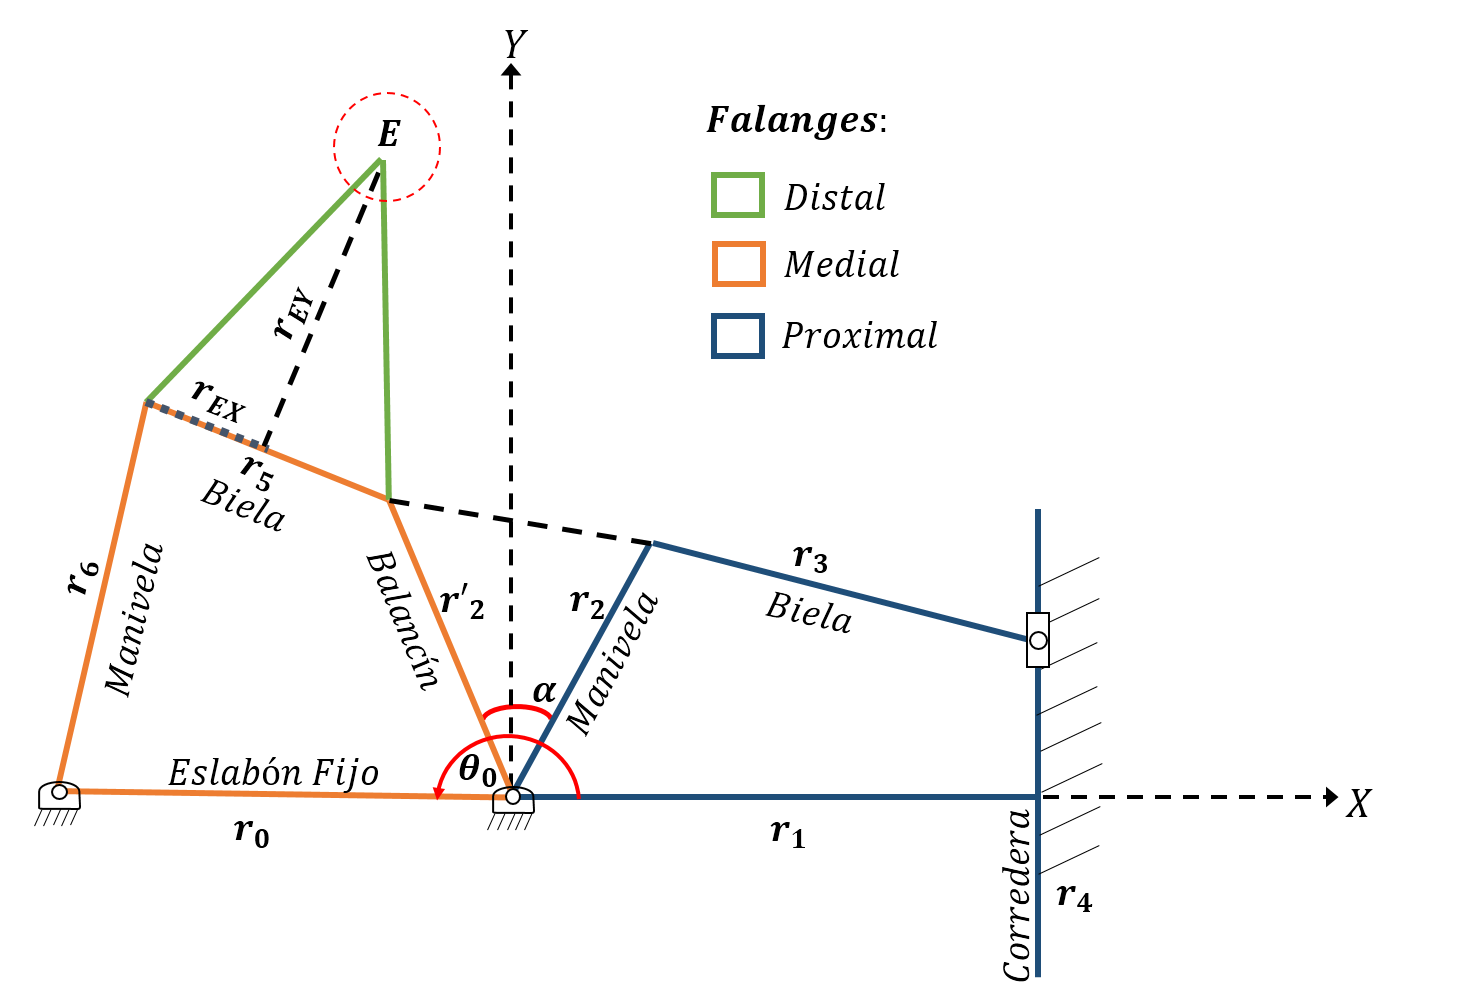
\includegraphics[width=0.9\textwidth]{Griper1.png}
    \caption [Mecanismo de seis barras para el diseño de un dedo del Efector Final.]{Mecanismo de seis barras para el diseño de un dedo del Efector Final. Tomado de \cite{zapata_zapata_control_2017} }
    \label{fig:Griper}
\end{figure}

En la Figura \ref{fig:Griper}, se muestra el diseño de un dedo conformado por dos sub-sistemas que simulan las falanges del mismo. El primer sub-sistema corresponde a un mecanismo manivela-biela-corredera (MBC) que se usa en la entrada ($r_2$, $r_3$, $r_4$), y el segundo es un mecanismo de cuatro barras en la salida ($r_0$, $r^{\prime}_2$, $r_5$, $r_6$). Ambos mecanismos conforman el sistema, en donde el impulsor es la corredera y el punto $E$ en el acoplador es la salida. El análisis de este problema fue tomado del trabajo realizado por Capistrán, Portilla y Mezura en \cite{capistran_2015} y se presenta en la siguiente sección.


\subsection{Cinemática del Efector Final de Tres Dedos }

Para llegar al planteamiento final de este problema de optimización se debe realizar primeramente el análisis de los dos sub-sistemas mencionados en la sección anterior individualmente. Luego, las ecuaciones que describen el comportamiento cinemático de ambos sistemas son integrados para conformar el problema de optimización. Primeramente se analiza el mecanismo MBC (Figura \ref{fig:Griper_MBC}) respecto al eje $X$ según la posición de la corredera $r_4$, en donde se pueden presentar tres casos posibles: $r_4 > 0$, $r_4 < 0$ y $r_4 = 0$. En cada caso la variable de interés que describe al sub-sistema es $\theta_3$. A continuación se presenta el modelo de cada caso \cite{capistran_2015}:
\begin{figure}[htb]
    \centering
     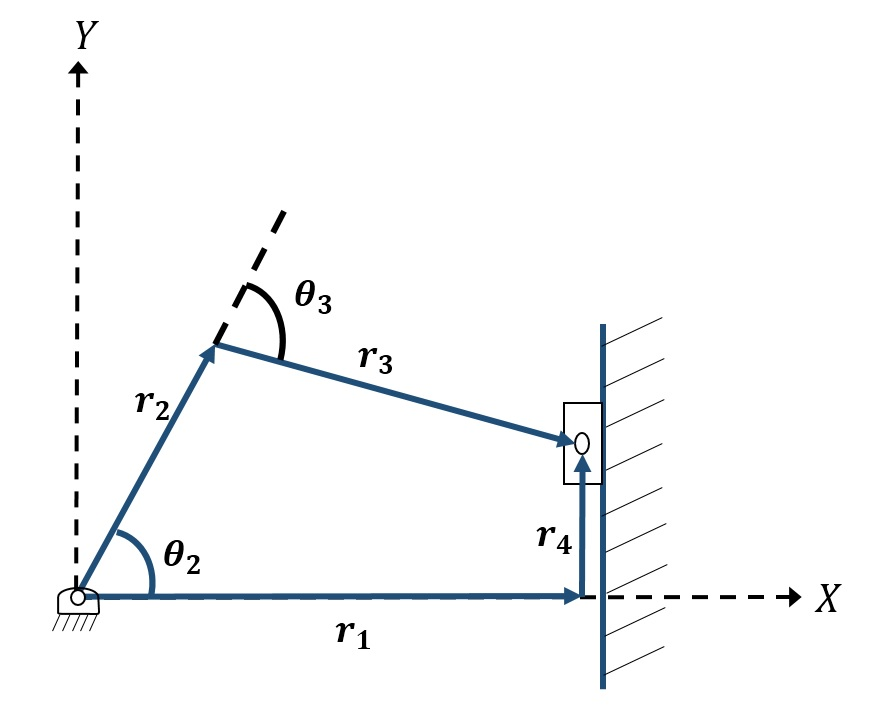
\includegraphics[width=0.8\textwidth]{Griper2.jpg}
    \caption[Mecanismo manivela-biela-corredera en un dedo del Efector Final.]{Mecanismo manivela-biela-corredera en un dedo del Efector Final. Tomado de \cite{zapata_zapata_control_2017} }
    \label{fig:Griper_MBC}
\end{figure}
\begin{enumerate}
\item \textbf{Si} $r_4>0$ \textbf{entonces}:

Se calcula el valor del ángulo $\theta_3$ mediante la sumatoria de los ángulos $\theta_2$, $\varphi$ y $\pi$  (igual a 180). En la Figura \ref{fig:Griper_MBC1} se muestran los ángulos requeridos para efectuar los cálculos necesarios en este caso.
\begin{figure}[htb]
    \centering
     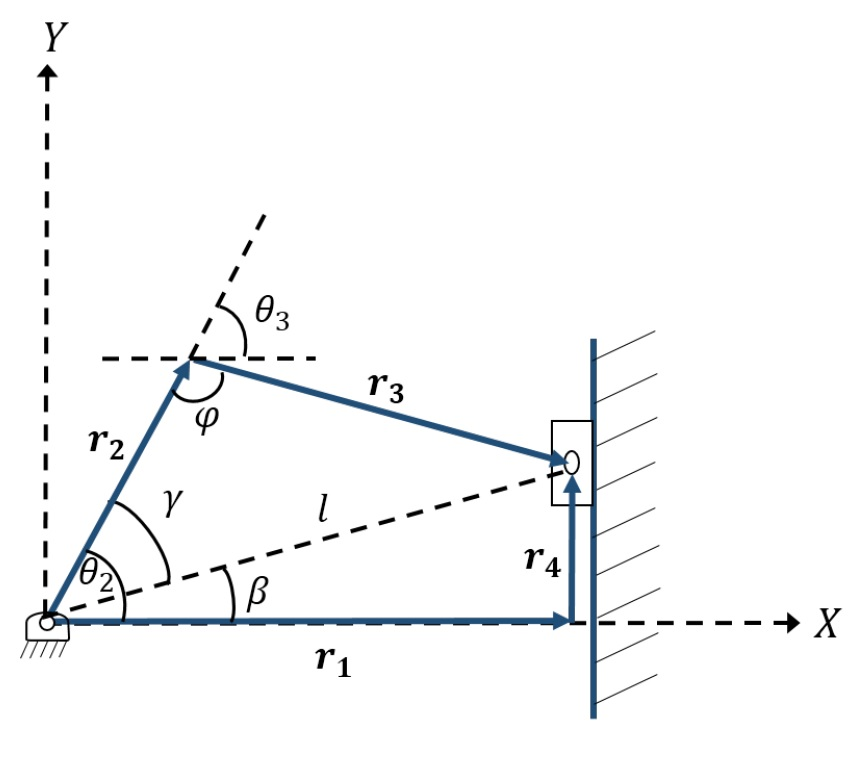
\includegraphics[width=0.8\textwidth]{Griper3.jpg}
    \caption [Mecanismo manivela-biela-corredera para $r_4 > 0$ en un dedo del Efector Final.]{Mecanismo manivela-biela-corredera para $r_4 > 0$ un dedo del el Efector Final. Tomado de \cite{zapata_zapata_control_2017} }
    \label{fig:Griper_MBC1}
\end{figure}

Para calcular $\theta_2$ se procede de la siguiente forma:
\begin{equation}\label{eq:griper_theta2}
\theta_2=\beta+\gamma
\end{equation}
Para obtener $\gamma$ debe calcular $l$ mediante el teorema de pitágoras:
\begin{equation}
l=\sqrt[]{r^2_1 +r^2_4}
\end{equation}
Aplicando la ley de cosenos y despejando se obtiene la Ecuación \ref{eq:griper_gamma} 
\begin{equation} \label{eq:griper_gamma}
\gamma=\cos^{-1}\left[  \frac{r^2_2 +l^2-r^2_3}{2r_2l}\right]
\end{equation}
Para cálculo  del ángulo se plantea que:
\begin{equation}\label{eq:griper_beta} 
\beta=\tan^{-1}\left[  \frac{|r_4|}{r_1}\right]
\end{equation}
Sustituyendo las Ecuaciones \ref{eq:griper_gamma} y \ref{eq:griper_beta} en la Ecuación \ref{eq:griper_theta2} se obtiene:
\begin{equation}\label{eq:griper_theta22}
\theta_2=  \cos^{-1}\left[  \frac{r^2_2 +l^2-r^2_3}{2r_2l}\right]+ \tan^{-1}\left[  \frac{|r_4|}{r_1}\right]
\end{equation}
El valor de $\varphi$ se calcula aplicando ley de cosenos y se despejando:
\begin{equation}\label{eq:griper_varphi}
\varphi=\cos^{-1}\left[ \frac{r^2_2 +r^2_3-l^2}{2r_2r_3}\right]
\end{equation}
Luego, el valor de $\theta_3$ se calcula por la sumatoria expresada en la Ecuación \ref{eq:griper_theta3}
\begin{equation}\label{eq:griper_theta3}
\theta_3=\theta_2+\varphi+\pi
\end{equation}
Esto es:
\begin{equation}\label{eq:griper_theta32}
\theta_3= \cos^{-1}\left[  \frac{r^2_2 +l^2-r^2_3}{2r_2l}\right]+ \tan^{-1}\left[  \frac{|r_4|}{r_1}\right]+\cos^{-1}\left[ \frac{r^2_2 +r^2_3-l^2}{2r_2r_3}\right]+\pi
\end{equation}
%%%%%%%%%%%%%%%%%%%%%%%%%%%

\item \textbf{Si} $r_4<0$ \textbf{entonces}:
\begin{figure}[htb]
    \centering
     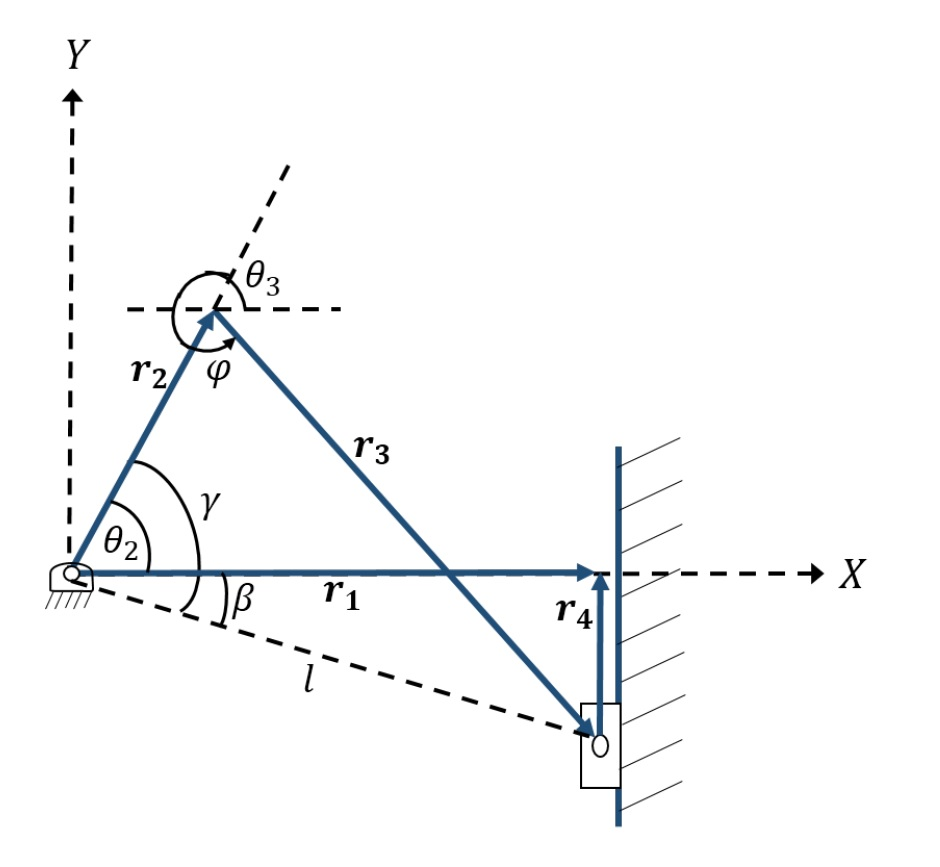
\includegraphics[width=0.8\textwidth]{Griper4.jpg}
    \caption [Mecanismo manivela-biela-corredera para $r_4<0$ en un dedo del Efector Final.]{Mecanismo manivela-biela-corredera para $r_4<0$ en un dedo del Efector Final. Tomado de \cite{zapata_zapata_control_2017} }
    \label{fig:Griper_MBC2}
\end{figure}

De forma similar al caso anterior el análisis matemático es similar al del caso anterior, se debe calcular el valor del ángulo $\theta_3$ solo que, en este caso el ángulo $\theta_2$ es la diferencia entre los ángulos $\beta$ y $\gamma$:
\begin{equation}\label{eq:griper_theta23}
\theta_2=\beta-\gamma
\end{equation}

Sustituyendo las Ecuaciones \ref{eq:griper_gamma} y \ref{eq:griper_beta} en la Ecuación \ref{eq:griper_theta23} se obtiene:
\begin{equation}\label{eq:griper_theta24}
\theta_2=  \cos^{-1}\left[  \frac{r^2_2 +l^2-r^2_3}{2r_2l}\right]- \tan^{-1}\left[  \frac{|r_4|}{r_1}\right]
\end{equation}

Luego, el valor de $\theta_3$ se obtiene sustituyendo este valor de $\theta_2$  y el valor de $\varphi$ de la Ecuación \ref{eq:griper_varphi},  en la Ecuación \ref{eq:griper_theta3}:
\begin{equation}\label{eq:griper_theta34}
\theta_3= \cos^{-1}\left[  \frac{r^2_2 +l^2-r^2_3}{2r_2l}\right]- \tan^{-1}\left[  \frac{|r_4|}{r_1}\right]+\cos^{-1}\left[ \frac{r^2_2 +r^2_3-l^2}{2r_2r_3}\right]+\pi
\end{equation}
%%%%%%%%%%%%%%%%%%%%%%%%%%

\item \textbf{Si} $r_4=0$ \textbf{entonces}:
\begin{figure}[htb]
    \centering
     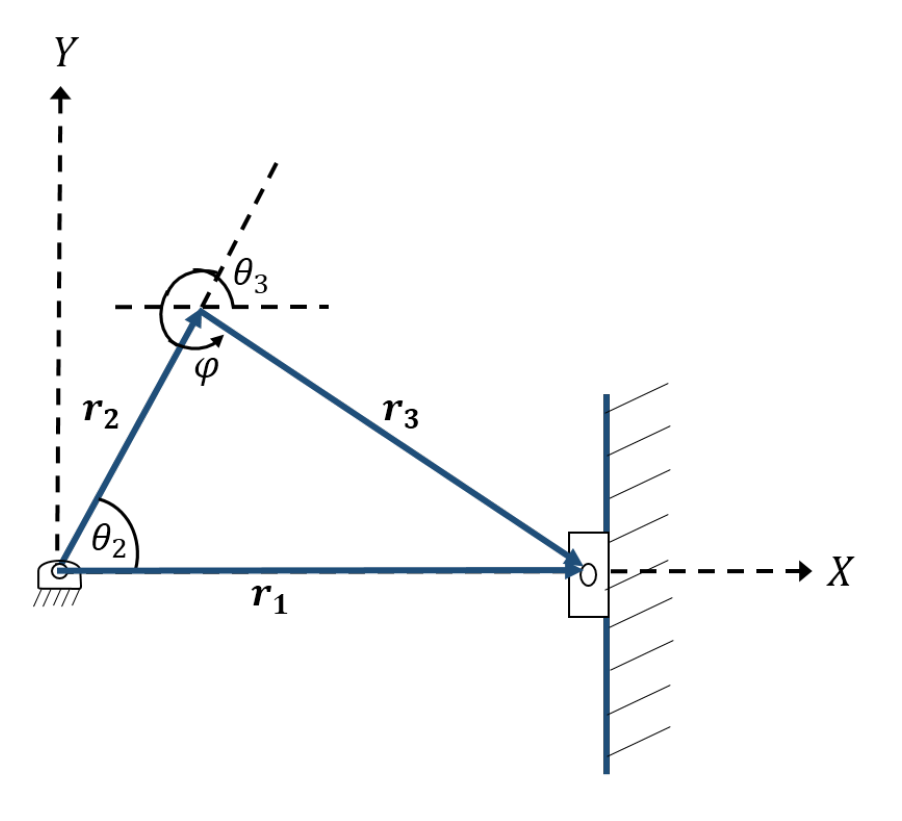
\includegraphics[width=0.8\textwidth]{Griper6.png}
    \caption[Mecanismo manivela-biela-corredera para $r_4 =0$ en un dedo del Efector Final.]{Mecanismo manivela-biela-corredera para $r_4 =0$ en un dedo del Efector Final. Tomado de \cite{zapata_zapata_control_2017} }
    \label{fig:Griper_MBC3}
\end{figure}

Debido que $r_4 = 0$ corredera del mecanismo se alinea con el eje $x$. Al igual que en los casos anteriores el valor del ángulo $\theta_3$ es igual a la suma de los ángulos $\theta_2$, $\varphi$ y $\pi$ . Para el calculo de $\theta_2$y $\varphi$ se aplica la ley de cosenos y se despeja, obteniendo las Ecuaciones \ref{eq:griper_theta25} y \ref{eq:griper_varphi3}
\begin{equation}\label{eq:griper_theta25}
\theta_2=\cos^{-1}\left[ \frac{r^2_1 +r^2_2-r^2_3}{2r_1r_2}\right]
\end{equation}
\begin{equation}\label{eq:griper_varphi3}
\varphi=\cos^{-1}\left[ \frac{r^2_2 +r^2_3-r^2_1}{2r_2r_3}\right]
\end{equation}
Finalmente, se sustituyen los ángulos $\theta_2$ y $\varphi$  en la Ecuación \ref{eq:griper_theta3}:
\begin{equation}\label{eq:griper_theta33}
\theta_3=\cos^{-1}\left[ \frac{r^2_1 +r^2_2-r^2_3}{2r_1r_2}\right]+\cos^{-1}\left[ \frac{r^2_2 +r^2_3-r^2_1}{2r_2r_3}\right]+\pi
\end{equation}

\end{enumerate}
El análisis cinemático presentado hasta el momento corresponde al sub-sistema MBC del mecanismo de seis barras. A continuación se procede a  desarrollar el modelo cinemático del mecanismo de cuatro barras conformado por los eslabones $r_0$, $r^{\prime}_2$, $r_5$ y $r_6$. En la Figura \ref{fig:Griper_MEC} se muestra dicho mecanismo sin el acoplador. Nótese, que la barra $r_2$ del sub-sistema MBC también forma parte del mecanismo de cuatro barras fungiendo como su impulsor y formando junto con $r^{\prime}_2$ un único eslabón.

\begin{figure}[htb]
    \centering
     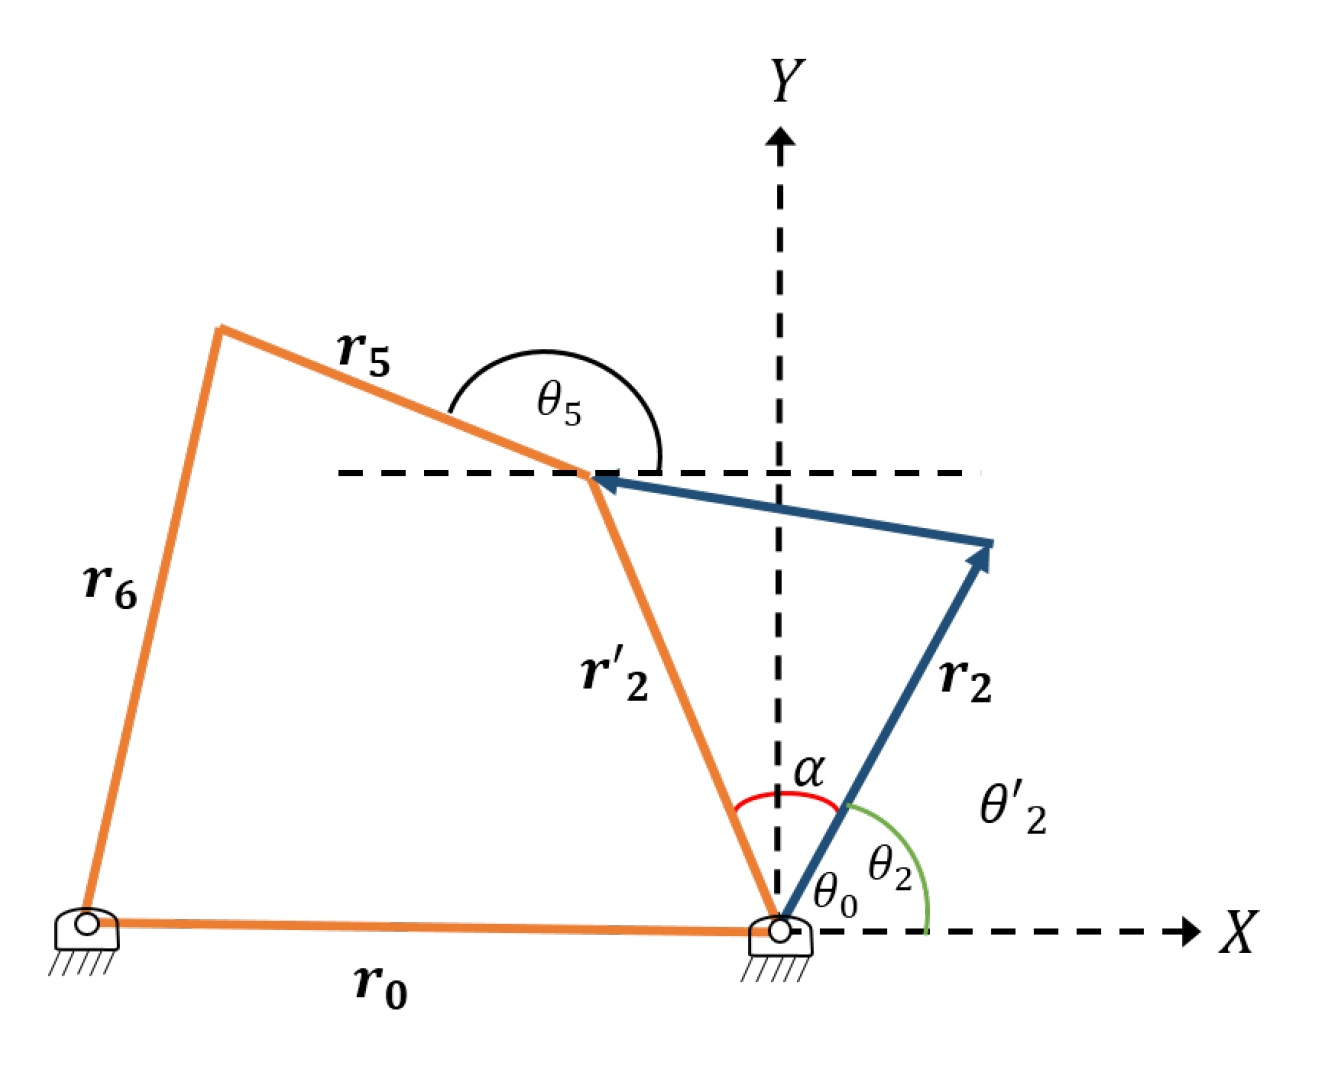
\includegraphics[width=0.8\textwidth]{Griper7.jpg}
    \caption [Mecanismo de cuatro barras de un dedo del Efector Final.]{Mecanismo de cuatro barras de un dedo del Efector Final. Tomado de \cite{zapata_zapata_control_2017} }
    \label{fig:Griper_MEC}
\end{figure}
El análisis cinemático del sub-sistema de cuatro barras es similar al del problema descrito en la Sección \ref{sec:Análisis cinemático de un Mecanismo de Cuatro Barras}. Para iniciar se establece la ecuación de lazo cerrado:
\begin{equation}\label{eq:griper_lazo}
\vec{r^{\prime}_2}+\vec{r_5}=\vec{r_0}+\vec{r_6}
\end{equation}
Utilizando la notación polar se tiene que:
\begin{equation}\label{eq:griper_lazoPolar}
r^{\prime}_2e^{j\theta^{\prime}_2}+r_5e^{j\theta_5}=r_0e^{j\theta_0}+r_6e^{j\theta_6}
\end{equation}
Aplicando la ecuación de Euler y separando la parte real de la parte imaginaria se obtiene:
\begin{eqnarray}
r^{\prime}_2 \cos{\theta^{\prime}_2}+r_5\cos{\theta_4}&=&r_0\cos{\theta_2} +r_6\cos{\theta_6} \label{eq:griper_PolarEuler5} \\
r^{\prime}_2 \sin{\theta^{\prime}_2}+r_5\sin{\theta_4} &=&r_0\sin{\theta_2}+r_6\sin{\theta_6}\label{eq:griper_PolarEuler6}
\end{eqnarray}
en donde:
\begin{equation}
\theta^{\prime}_2=\theta_2+\alpha
\end{equation}
El ángulo $\theta_2$ se obtiene del análisis cinemático del sub-sistema MBC. Luego para calcular $\theta_5$, el sistema de ecuaciones \ref{eq:griper_PolarEuler5} se expresa en función de $\theta_4$ para obtener:
\begin{eqnarray}
r_6\cos{\theta_6}&=& r^{\prime}_2\cos{\theta^{\prime}_2}+r_5\cos{\theta_5}-r_0\cos{\theta_0}\label{eq:griper_PolarEuler7} \\
r_6\sin{\theta_6} &=&r^{\prime}_2\sin{\theta^{\prime}_2}-r_5\sin{\theta_5}r_0\cos{\theta_0}\label{eq:griper_PolarEuler8}
\end{eqnarray}
Se obtiene la ecuación compacta de Freudenstein elevando al cuadrado los términos del sistema de ecuaciones anterior y sumando sus términos:
\begin{equation} \label{eq:griper_A1B1C1}
 A\cos{\theta_3}+B\sin{\theta_3}+C=0 
\end{equation}
Donde:
\begin{eqnarray}
A&=& 2r_5(r^{\prime}_2\cos{\theta^{\prime}_2}-r_0\cos{\theta_0}) \label{eq:griper_A} \\
B&=& 2r_5(r^{\prime}_2\sin{\theta^{\prime}_2}-r_0\sin{\theta_0}) \label{eq:griper_B} \\
C&=& r_0^2+r^{\prime}_2+r_5^2-r_6^2 -2r_0r^{\prime}_2\cos(\theta_0-\theta^{\prime}_2) \label{eq:griper_C}
\end{eqnarray}
El ángulo $\theta_5$ se puede obtener como función de $A$, $B$ y $C$, si $\sen{\theta_5}$ y $\cos{\theta_5}$  se expresan en términos de $\tan(\frac{\theta_5}{2})$:
\begin{eqnarray}
\sin{\theta_5}= \frac{2tan(\frac{\theta_5}{2})}{1+tan^2(\frac{\theta_5}{2})}&,& \cos{\theta_5}= \frac{1-tan^2(\frac{\theta_5}{2})}{1+tan^2(\frac{\theta_5}{2})} \label{eq:griper_enFuncionTheta3}
\end{eqnarray}

Sustituyendo la Ecuación \ref{eq:griper_enFuncionTheta3} en la Ecuación \ref{eq:griper_A1B1C1} se obtiene una ecuación no lineal de segundo orden:
\begin{equation} \label{eq:griper_Lineal2dOrden}
 \left[C-A\right]= tan^2{\frac{\theta_3}{2}}+\left[2B\right]\tan{(\frac{\theta_3}{2})}+A+C=0
\end{equation}
Resolviendo la ecuación \ref{eq:griper_Lineal2dOrden} el ángulo $\theta_3$ puede ser expresado de la siguiente forma:
\begin{equation} \label{eq:griper_noLineal2dOrden_theta5}
\theta_5= 2\arctan \left[ \frac{-B \pm \sqrt{B^2+A^2-C^2}}{C-A} \right]
\end{equation}
El ángulo $\theta_6$ se obtiene de forma similar, siendo la ecuación compacta de Freudenstein:
\begin{equation} \label{eq:griper_A1B1C1_2}
 D\cos{\theta_6}+E\sin{\theta_6}+F=0 
\end{equation}
Donde:
\begin{eqnarray}
D&=& 2r_6(r_0\cos{\theta_0}-r^{\prime}_2\cos{\theta^{\prime}_2}) \label{eq:griper_A_2} \\
E&=& 2r_6(r_0\sin{\theta_0}-r^{\prime}_2\cos{\theta^{\prime}_2}) \label{eq:griper_B_2} \\
F&=& r_0^2+r^{\prime}_2+r_5^2-r_6^2 -2r_0r^{\prime}_2\cos(\theta_0-\theta^{\prime}_2) \label{eq:griper_C_2}
\end{eqnarray}
Luego, $\theta_6$ se define como:
\begin{equation} \label{eq:griper_noLineal2dOrden_theta6}
\theta_6= 2\arctan \left[ \frac{-E \pm \sqrt{E^2+D^2-F^2}}{F-D} \right]
\end{equation}
Las Ecuaciones \ref{eq:griper_noLineal2dOrden_theta5} y \ref{eq:griper_noLineal2dOrden_theta6} determinan los ángulos de la biela y el balancín del mecanismo de cuatro barras. El signo del radical para los ángulos $\theta_5$ y $\theta_6$ también se seleccionan de acuerdo a la la Tabla \ref{tab:Signo del radical} de la Sección \ref{sec:Análisis cinemático de un Mecanismo de Cuatro Barras}. Para analizar, se debe determinar la posición del punto $E$ del acoplador (Figura \ref{fig:Griper_MEC1}) a través de la siguiente relación:
\begin{equation} \label{eq:griper_E}
E=r^{\prime}_2+ r_{EX}+r_{EY}
\end{equation}
En términos de componentes tenemos que:
\begin{eqnarray}
E_{x}&=&r^{\prime}_2\cos{\theta^{\prime}_2} +r_{EX}\cos{\theta_5}+r_{EY}\sin{\theta_{EY}} \label{eq:gripper_Cxr} \\
E_{y}&=&r^{\prime}_2\cos{\theta^{\prime}_2} +r_{EY}\sin{\theta_5}+r_{EY}\cos{\theta_{EY}}\label{eq:gripper_Cyr}
\end{eqnarray}
en donde:
\begin{eqnarray}
\theta^{\prime}_{2} &=& \theta_2-\alpha \\
\theta_{EY} &=& \theta_5-90
\end{eqnarray}

\begin{figure}[htb]
    \centering
     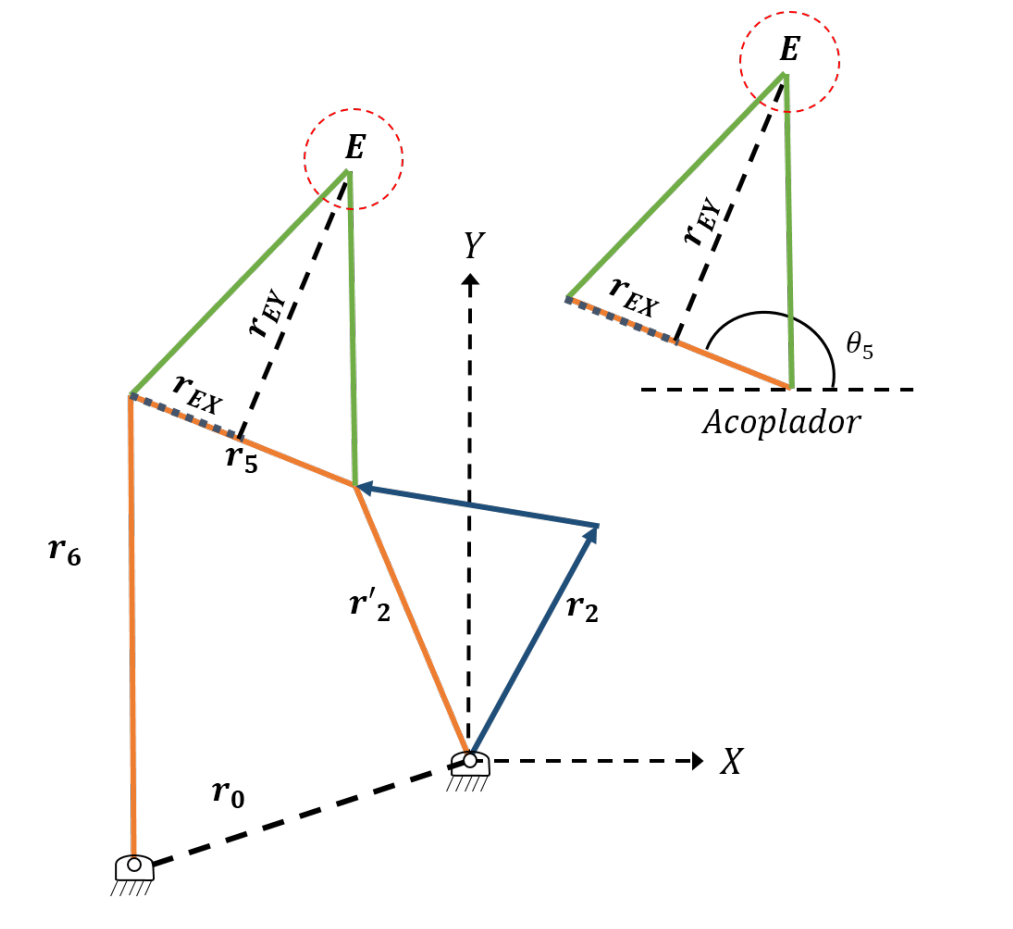
\includegraphics[width=0.8\textwidth]{Griper8.png}
    \caption[Acoplador del mecanismo de cuatro barras en un dedo del Efector Final]{Acoplador del mecanismo de cuatro barras en un dedo del Efector Final. Tomado de \cite{zapata_zapata_control_2017} }
    \label{fig:Griper_MEC1}
\end{figure}
\subsection{Declaración de Problemas de Optimización para Casos de Estudio del Efector}
Para la optimización del diseño correspondiente a un dedo del efector final, se deben encontrar las dimensiones de todas los eslabones del mecanismo de seis barras de tal forma que el punto E del acoplador siga una trayectoria esferica. Los puntos de la trayectoria se encuentran definidos por la Ecuación \ref{eq:griper_puntosP} y fueron tomados de \cite{capistran_2015}.
\begin{equation} \label{eq:griper_puntosP}
 \Omega= \left\{(10, 160), (10, 170), (40, 165) \right\}
\end{equation}
El vector de variables para este caso está constituido por 14 componentes:
\begin{eqnarray}\label{eq:gripper_Vector variables MEC1}
\vec{p} &=& \{p_1,p_2,p_3,...,p_{14} \}\\
       &=& \{ r_1,r_2,r_3,r^1_4,r^2_4,r^3_4,r_0,r^{\prime}_2,r_5,r_6,r_{EX},r_{EY},\alpha,\theta_0 \} 
\end{eqnarray}
En donde $r_1$, $r_2$, $r_3$, $r_0$, $r^{\prime}_2$, $r_5$ y $r_6$ son las dimensiones de las barras. Las variables $r^1_4$,$r^2_4$,$r^3_4$, corresponden a las posiciones de la corredera y se emplean para calcular los puntos en los que se ubica el sistema, $r_{EX}$ y $r_{EY}$ son las dimensiones de las barras del acoplador, mientras que  $\alpha$ es el ángulo entre $r_2$ y $r^{\prime}_2$ , y $\theta_0$ el ángulo de $r_0$.
\subsubsection{Función objetivo}
Para el primer caso del efector final  se plantea la función de error 
\begin{equation}
 \begin{aligned}
min\quad  f(r^i_4)=\sum_{i=1}^{N}\big[\big(C^{i}_{1d}-C^{i} \big)^2=
\sum_{i=1}^{N}\big[\big(C^{i}_{1xd}-C^{i}_{x} \big)^2 +\big(C^{i}_{yd}-C^{i}_{y} \big)^2\big] 
\end{aligned}
\label{eq:gripper_FO}
\end{equation}
En la Ecuación \ref{eq:gripper_FO} se calcula la distancia (a minimizar) de los puntos de precisión $C^i_d$ y los puntos calculados $C_i$ a partir de $r^i_4$. Donde  $C^i_x$ y $C^i$ son las coordenadas $(x,y)$ del punto $E$ del acoplador.
\subsubsection{Restricciones de diseño}\label{sec:Restricciones de diseño MEC_gripper}
Para el correcto funcionamiento del gripper se deben tener en cuenta las siguientes restricciones de diseño: 
\begin{itemize}
\item \textit{Ley de Grashof:} De forma similar al mecanismo de 4 barras, debe cumplirse la ley de Grashof para el mecanismo de seis barras:
\begin{equation}
r_5+r_6 \leq r_0+r^{\prime}_2
\end{equation}
Adicionalmente debe cumplirse que:
\begin{equation}
r_0<r_6, \quad r^{\prime}_2<r_6 ,\quad r_5 < r_6
\end{equation}

\item \textit{Secuencia de posición de la corredera}: Las  posiciones de la corredera deben estar ordenadas de tal forma que cada posición preceda a la siguiente de acuerdo a su magnitud:
\begin{equation}
r^1_4 > r^2_4 > r^3_4
\end{equation}

\item \textit{Consideraciones sobre barras}: Esta restricción tiene como objetivo garantizar un alto nivel que la estética del acoplador. Para lograr esto $r_{EX}$ debe ser lo más parecida posible a $r_5$, por lo que: 
\begin{equation}
 r_{EX} - r_5 \leq 0
\end{equation}
Además, para el sub-sistema MBC, la relación recomendada entre biela y manivela se encuentra entre $\frac{1}{3}$ y $\frac{1}{5}$, esto es:
\begin{equation}
\frac{1}{5} \leq \frac{r_2}{r_3}\leq \frac{1}{3}
\end{equation}
Luego:
\begin{equation}
r_2 -\frac{r_3}{3} \leq 0 \quad , \quad \frac{r_3}{5} -r_2 \leq 0
\end{equation}
\end{itemize}

Finalmente, se formulan en las siguientes secciones dos casos de estudio para  el diseño óptimo del gripper, ambos comparten el mismo vector de variables y el conjunto de puntos de precisión.
\subsection{Caso de estudio 1: Diseño sin normalización de barras -GCE1}

El problema de optimización mono-objetivo para el este caso de estudio se define como:
 \begin{equation}\label{eq:gripper_FO1}
 \begin{aligned}
min\quad  f(\vec{p})=
\sum_{i=1}^{3}\big[\big(C^{i}_{xd}-C^{i}_{x} \big)^2 +\big(C^{i}_{yd}-C^{i}_{y} \big)^2\big]
\\
\vec{p} \in  {\rm I\!R}^{15}
\\
\end{aligned}
\end{equation}
%1 () =  ⃗ 1 + 2 − 3 − 4 ≤ 0,
s.a:
\begin{eqnarray}\label{eq:Restricciones gripper1}
g_{1}(\vec{p})&=&p_{10}+ p_{9}-p_{8}-p_{7} \leq 0,\\
g_{2}(\vec{p})&=&p_{7}-p_{10} \leq 0,\\
g_{3}(\vec{p})&=&p_{8}-p_{10} \leq 0,\\
g_{4}(\vec{p})&=&p_{9}-p_{10} \leq 0,\\
g_{5}(\vec{p})&=&p_{11}-p_{9} \leq 0,\\
g_{6}(\vec{p})&=&|p_{4}|-|p_{5}| \leq 0,\\
g_{7}(\vec{p})&=&|p_{5}|-|p_{6}| \leq 0,\\
g_{8}(\vec{p})&=&p_{2}-\frac{p_3}{3} \leq 0,\\
g_{9}(\vec{p})&=&\frac{p_3}{3}-p_{2} \leq 0
\end{eqnarray}
Los límites superior e inferior de cada variable de diseño son los siguientes:
\begin{eqnarray}\label{eq:limites variables griper1}
p_1,p_2,p_3 & \in & \left[ 0,100\right] \\
p_4,p_5,p_6 & \in & \left[ -50,0\right] \\
p_7,p_8,p_{10},p_{11},p_{12} & \in & \left[ 0,150 \right] \\
p_9 & \in & \left[ 0,50\right] \\
p_{13} & \in & \left[ \frac{\pi}{12},\pi \right] \\
p_{14} & \in & \left[ \frac{3\pi}{4},\frac{5\pi}{4} \right]
\end{eqnarray}
\subsection{Caso de estudio 2: Diseño con normalización de barras - GCE2}

En el segundo caso de estudio se agrega una función de normalización ($f(\vec{x})$) para las barras del mecanismo, con el fin de obtener un diseño  estético y antropomórfico de las falanges del gripper. La función objetivo queda definida de la siguiente forma:
\begin{equation}\label{eq:griper_FOG1}
  f_r= w_1f(\vec{p})+w_2f(\vec{x})
\end{equation}
esto es:
 \begin{eqnarray}\label{}
min\quad  f(\vec{p})&=&
\sum_{i=1}^{3}\big[\big(C^{i}_{xd}-C^{i}_{x} \big)^2 +\big(C^{i}_{yd}-C^{i}_{y} \big)^2\big] \qquad \vec{p} \in  {\rm I\!R}^{14} \\
min\quad  f(\vec{x})&=&\frac{\sqrt[]{\sum^6_{i=1}\sum_{j=1}(x_j-x_i)^2}}{\sqrt[]{\sum^6_{i=1}x^2_i}} \label{eq:griper_NORM}
\end{eqnarray}
%1 () =  ⃗ 1 + 2 − 3 − 4 ≤ 0,
s.a:
\begin{eqnarray}\label{eq:Restricciones griper2}
g_{1}(\vec{p})&=&p_{10}+ p_{9}-p_{8}-p_{7} \leq 0,\\
g_{2}(\vec{p})&=&p_{7}-p_{10} \leq 0,\\
g_{3}(\vec{p})&=&p_{8}-p_{10} \leq 0,\\
g_{4}(\vec{p})&=&p_{9}-p_{10} \leq 0,\\
g_{5}(\vec{p})&=&p_{11}-p_{9} \leq 0,\\
g_{6}(\vec{p})&=&|p_{4}|-|p_{5}| \leq 0,\\
g_{7}(\vec{p})&=&|p_{5}|-|p_{6}| \leq 0,\\
g_{8}(\vec{p})&=&p_{2}-\frac{p_3}{3} \leq 0,\\
g_{9}(\vec{p})&=&\frac{p_3}{3}-p_{2} \leq 0
\end{eqnarray}
Los límites superior e inferior para las variables de diseño son:
\begin{eqnarray}\label{eq:limites variables griper2}
p_1,p_2,p_3 & \in & \left[ 0,100\right] \\
p_4,p_5,p_6 & \in & \left[ -50,0\right] \\
p_7,p_8,p_{10},p_{11},p_{12} & \in & \left[ 0,150 \right] \\
p_9 & \in & \left[ 0,50\right] \\
p_{13} & \in & \left[ \frac{\pi}{12},\pi \right] \\
p_{14} & \in & \left[ \frac{3\pi}{4},\frac{5\pi}{4} \right]
\end{eqnarray}
En la Ecuación \ref{eq:griper_FOG1}, $w_1$ y $w2$ , son pesos que controlan la precisión de la trayectoria y la estética del mecanismo, respectivamente. La suma de ambos pesos debe ser igual 1, por lo que, para este caso se tomarán los valores de $w_1=0.9$ y $w_2=0.1$. Las variables $x_i$ y $x_j$ de la Ecuación \ref{eq:griper_NORM} están relacionadas con las coordenadas de cada barra del sistema.

\section{Gestión de Generación de Energía en una Microrred Eléctrica}
En la actualidad los sistemas de generación y distribución de energía convencionales enfrentan diversos problemas como el agotamiento gradual de los recursos de combustibles fósiles, la escasa eficiencia energética y la contaminación ambiental. Estos problemas han impulsado la nueva tendencia de generar energía localmente mediante el uso de \textit{Fuentes de Energía Renovables} (FER) como gas natural, biogás, energía eólica, panales solares fotovoltaicos, sistemas combinados de calor y energía, y su integración en la red de distribución energía de uso público. Este tipo de generación de energía se denomina \textit{generación distribuida} (GD) y las fuentes de energía se denominan\textit{ recursos de energía distribuida }(RED). El término generación distribuida se utiliza para distinguir este concepto de generación convencional centralizada. Debido al aumento tanto de la demanda de energía eléctrica como del uso las FER, la utilización de microrredes eléctricas ha tenido un aumento en las ultimas décadas. Lasseter plantea lo siguiente en  \cite{lasseter2002microgrids}:
\begin{quote}
\textit{``Las microrredes son redes de suministro de energía de pequeña escala, diseñadas para suministrar cargas eléctricas o térmicas a una comunidad pequeña, como una urbanización o una localidad suburbana. Una Microrred es esencialmente una red de distribución ya que es un conglomerado de sistemas GD con diferentes cargas a nivel de voltaje de distribución. Los generadores o micro-fuentes empleados en una Microrred suelen ser de Generación Distribuida renovable o no convencional."}
\end{quote}


Desde el punto de vista operativo, las micro-fuentes deben estar equipadas con interfaces electrónicas de potencia (IEP) y controles para proporcionar la flexibilidad requerida y  garantizar así el funcionamiento como sistema único. Esta flexibilidad de control permite que la Micro-red se presente al sistema de energía de la red principal como una sola unidad controlada que satisface las necesidades locales de energía. La principal ventaja de una Microrred es su facilidad de control, así como el cumplimiento de las regulaciones de la red sin obstaculizar la confiabilidad y seguridad del servicio eléctrico. Desde el punto de vista de los clientes, las microrredes son beneficiosas para satisfacer localmente sus requisitos eléctricos. Pueden suministrar energía ininterrumpible, mejorar la confiabilidad local y proporcionar soporte de voltaje local. Desde el punto de vista ambiental, las microrredes reducen la contaminación ambiental y el calentamiento global mediante la utilización de tecnología que produce bajas emisiones de carbono  \cite{lasseter2002microgrids}. 

Sin embargo, para lograr una operación estable y segura mediante micro-redes, es necesario resolver una serie de problemas técnicos, normativos y económicos. Ciertas características de las microrredes pueden resultar problemáticas. Algunas intrínsecas, como la naturaleza intermitente y dependiente del clima de la generación mediante ciertos tipos de FER como la fotovoltaica y la eólica; u otras como el bajo contenido de energía de los combustibles no fósiles, la falta de estándares y regulaciones para operar las Microrredes de forma factible. El estudio de estas cuestiones requiere un amplio análisis en tiempo real y en simulaciones, que ha sido objeto de diferentes investigaciones.

 \subsection{Optimización del costo de la generación de energía en una Microrred Eléctrica No Interconectable - SCE1}
En el presente problema el objetivo es minimizar el costo de operación de una  Microrred Eléctrica en un lugar remoto no interconectable (MR-RNI), al tiempo que se garantiza el equilibrio entre la generación y la demanda. La generación fiable de energía se logra mediante la generación híbrida de potencia en donde se emplean Fuentes de Energía Renovables (FER), generación convencional con diésel y Sistemas de Almacenamiento de Energía (SAE). Las variables de diseño representan entonces, las potencias que serán suministradas por los Generadores de Diésel (GD), energía fotovoltáica (GFV), energía eólica (GE) y el  de la MR-RNI en función del tiempo dentro de un intervalo de 24 horas. Se define un modelo de optimización basado en el despacho económico, el cual intenta obtener el menor costo posible derivado del uso del sistema, mientras los generadores entregan potencia a la carga total. El cálculo de minimización del costo de la generación de energía  eléctrica en la MR-RNI se debe realizar para un periodo de 24, donde cada hora del día representa un problema de optimización con límites para las variables de diseño diferentes en cada hora. Esto se debe a que los recursos para la generación diaria son variables. Específicamente debe tomarse en cuenta los siguientes escenarios \cite{zapata_zapata_control_2017}: 
\begin{enumerate}
\item Las FER no pueden entregar energía las 24 horas.
\item La demanda total de energía no puede ser entregada solo por las FER.
\item Los costos más representativos son los de combustible,y por tanto la potencia entregada por el generador de diésel es la más costosa.
\item La operación de los sistemas de generación híbrida de potencia tiene un costo generalmente no lineal.
\end{enumerate}
\subsubsection{Costo de Generación Diésel}
La GD presenta una función de costo asociada a la potencia del generador. Dicha función se encuentra dada por la Ecuación \ref{eq:GD}, en donde $i$ es la $i$-ésima fuente de generación , $P_i$ y $F_i$ son la salida de potencia eléctrica y el costo de operación de la fuente $i$, respectivamente, mientras que $\alpha$, $\beta$  y $\gamma$ son los cocientes de costo.
 \begin{equation}\label{eq:GD}
   f(P_i)=\alpha_i +\beta_iP_i +\gamma P^2_i
 \end{equation}
Para  $\alpha=14.88$, $\beta=0.3$  y $\gamma=0.000435$ según se plantea en \cite{zapata_zapata_control_2017}. Luego la función de costo correspondiente a la generación de diésel se define entonces como:
 \begin{equation}\label{eq:GD1}
   f_1(P_1)=14.88 +0.3P_1 +0.000435 P^2_1
 \end{equation}

\subsubsection{Costo de Generación Solar Fotovoltaica}
Para el generador de energía fotovoltaica se define la siguiente función de costo de generación:
\begin{equation}\label{eq:PV1}
   f_3(P_3)=\alpha I^p P_3 +G^EP_3 
 \end{equation}
 
 \begin{equation}\label{eq:PV2}
  \alpha = \frac{r}{\left[1+(1+r)^{-N}\right]}
 \end{equation}

En este caso $P_3$ es la potencia de salida de GFV, $\alpha$ es la tasa de retorno de inversión y $r$ corresponde a la tasa de interés (se considera de 0.09 para el caso base), $N$ es la vida útil del generador, que ha sido establecida
en 20 años, $I^p$ indica el costo de inversión por unidad de potencia (\$5000=kW) y $G^E$ es el costo de operación y mantenimiento por unidad de potencia generada. La función de costo por generación fotovoltaica queda definida entonces como:
\begin{equation}\label{eq:PV3}
   f_3(P_3)=545.016P_3 
\end{equation}
\subsubsection{Costo de Generación de Energía Eólica}
Según lo planteado en \cite{zapata_zapata_control_2017} se toman los mismos
valores de $I^p$ y $G^E$, la función de costo para la generación eólica queda como:
\begin{equation}\label{eq:GE}
f_4(P_4) = 152.616P_4
\end{equation}
\subsubsection{Costo de Sistema de Almacenamiento de Energía}
Para el SAE se considera un banco de baterías de 2kW. En \cite{zapata_zapata_control_2017}, el costo $I^p$ por unidad de almacenamiento instalada es de \$1000/kW, mientras que el $G^E$ es igual a \cent 1.6/kW y representa el costo de operación y mantenimiento por unidad de potencia generada. El uso del SAE describe la siguiente función de costo:
\begin{equation}\label{eq:ESS}
f_2(P_2) = 119P_2
\end{equation}
\subsection{Planteamiento del Problema de Optimización}
El despacho económico es un método eficiente para obtener un menor costo del sistema al tiempo que se satisface la carga o demanda de energía mediante el despacho de las fuentes de generación. Simultáneamente, las restricciones de las fuentes de generación deben ser satisfechas. En el presente caso de estudio se deben calcular las potencias de cada uno de los generadores en la MR-RNI en cada hora del día, minimizando el costo. El vector de variables de diseño se plantea en la Ecuación  \ref{eq:MR-vector de variables}:
 \begin{equation}\label{eq:MR-vector de variables}
  \vec{p}=\left[ P_1,P_2,P_3,P_4 \right]^T
 \end{equation}


La formulación clásica del despacho económico se plantea en \cite{Ramabhotla_Economic_dispatch} de la siguiente forma:
 \begin{equation}
 min\quad  F=
 \sum_{i=1}^{NG}F_{i}P_{i} 
 \end{equation}

Donde $NG$ es el número de fuentes; $P_{i}$ es el generador de fuente $i$; $F_{i}$ es el costo total de producción de la fuente $i$. Luego la función objetivo considerada para el caso de estudio en cuestión tiene en cuenta la variabilidad de la carga en cada hora  $\tau$ del día según la Ecuación \ref{eq:MR-FO}
 \begin{equation}\label{eq:MR-FO}
min \quad f(\vec{p} ) = w_1C_f f(P_1(\tau)) + w_2f(P_2(\tau)) + w_3f(P_3(\tau))+ w_4f(P_4(\tau))
 \end{equation}
 
Donde $w_1$,$w_2$,$w_3$,$w_4$ son los pesos asignados a los generadores, cumpliéndose que  $w_1+ w_2+w_3+w_4=1$ y  se establece que $w_1=w_2=w_3=w_4=0.25$. $C_f$ es el costo del combustible de diésel que se asignó en 1 USD.


Teniendo en cuenta que el costo de generación de energía debe ser calculado en cada hora del día la función objetivo para las 24 horas del día se define según la Ecuación \ref{eq:MR-FO2}:
\begin{equation}\label{eq:MR-FO2}
 min\quad  F=
 \sum_{\tau=1}^{24}f(\vec{p}_\tau) \quad \vec{p}_\tau \in {\rm I\!R}^{4}
 \end{equation}
\subsubsection{Restricciones de Diseño}
La gestión de generación de energía en la MR-RNI está sujeta a las siguientes restricciones de diseño:
\begin{itemize}
\item \textit{Balance de potencia}: La suma de las potencias suministradas por los cuatro generadores debe ser igual a la carga $P_L$ del sistema :
 \begin{equation}
P_1+P_2+P_3+P_4=P_L
 \end{equation}
 \item \textit{Modelo del banco de baterías}: El poder de salida del generador PV y la carga demandada en cierta hora $t$, determinan el poder de carga y descarga dentro y fuera del banco de baterías.
El estado de carga ($SOC$ por sus siglas en inglés) del banco de baterías en cualquier hora, $SOC(t)$,depende del $SOC$ en la hora previa $SOC(t-1)$. Luego, para el flujo de energía de la hora $t-1$ a $t$, se debe considerar la siguiente relación \cite{tazvinga2013minimum}:
 \begin{equation}
SOC(t)=SOC(t-1)- \alpha_DP_2(t)+\alpha_CP_3(t)+\alpha_CP_4(t)
 \end{equation}
 Donde $\alpha_D=\frac{\eta_D}{Bc_{max}}$, $\alpha_C=\frac{\eta_C}{Bc_{max}}$ y $\eta_D$ y $\eta_D$ son las eficiencias de carga y descarga del banco de baterías respectivamente. Luego la expresión que describe la dinámica de la batería se define como \cite{tazvinga2013minimum}:
  \begin{equation}
SOC(t-1)=SOC(0)- \alpha_D \sum_{\tau=1}^{t}P_2(\tau)+\alpha_C\sum_{\tau=1}^{t}P_3(\tau)+\alpha_C \sum_{\tau=1}^{t}P_4(\tau)
 \end{equation}
 
donde se tiene que $SOC(0)$ como el $SOC$ inicial de la batería y  $\alpha_C\sum_{\tau=1}^{t}P_3(\tau)+\alpha_C \sum_{\tau=1}^{t}P_4(\tau)$ es el poder aceptado por la batería en la hora $t$ y  $\alpha_D \sum_{\tau=1}^{t}P_2(\tau)$ es el poder de descarga de la batería en el tiempo $t$.
Además se debe tener en cuenta que la capacidad disponible de la batería no debe ser menor que la capacidad mínima permitida ni mayor que la capacidad máxima permitida \cite{tazvinga2013minimum}, es decir:
\begin{equation}
SOC^{min}-SOC(t)\leq 0 \quad, \quad SOC(t)-SOC^{max}-\leq 0 
 \end{equation}
 Los parámetros del banco de baterías se muestran en la Tabla \ref{tab:MR-Parámetros del Sistemas de Almacenamiento de Energía}
\begin{table}[]
\centering
\begin{tabular}{ll}
\hline
 Parámetros &   \% \\ \hline
 Eficiencia de carga ($\eta_C$)  & 85 \\
 Eficiencia de descarga ($\eta_D$) & 100  \\
 Estado máximo de carga ($SOC_{max}$)& 95\\ 
 Estado mínimo de carga ($SOC_{min}$)& 40\\
 \hline
\end{tabular}
\caption{Parámetros del Sistemas de Almacenamiento de Energía en la Micro-Red No Interconectable.}
\label{tab:MR-Parámetros del Sistemas de Almacenamiento de Energía}
\end{table}

\end{itemize}
Teniendo en cuenta las secciones anteriores, se plantea el problema de optimización mono-objetivo para el caso de estudio de la MR-RNI descrito por las Ecuaciones de la \ref{eq:MR-FO3} a la \ref{eq:ultima restriccion MR}:

\begin{equation}\label{eq:MR-FO3}
 min\quad  F=
 \sum_{\tau=1}^{24}f(\vec{p}_\tau) \quad \vec{p}_\tau \in {\rm I\!R}^{4}
 \end{equation}
 s.a:
\begin{eqnarray}\label{eq:Restricciones MR}
g_1(\vec{p}_\tau)&=&P_1(\tau)+P_2(\tau)+P_3(\tau)+P_4(\tau)=P_L(\tau)\\
g_2(\vec{p}_\tau)&=&SOC^{min}-SOC(t)\leq 0 \\
g_3(\vec{p}_\tau)&=&SOC(t)-SOC^{max}-\leq 0 
\end{eqnarray}
La carga $P_L(\tau)$ fue obtenida de \cite{tazvinga2014energy} y los límites superior e inferior de cada variable se encuentran definidos como:
\begin{eqnarray}\label{eq:Restricciones MR3}
0  & \leq & P_1(\tau)   \leq  GD_{nominal} \\
0  & \leq & P_2(\tau)   \leq  SOC(0) \times Bc_{max}-  SOC^{min} \times  Bc_{max}\\
0  & \leq & P_3(\tau)   \leq  P_{pv}( \tau) \\
0  & \leq & P_4(\tau)   \leq  P_{wind}(\tau )  \label{eq:ultima restriccion MR}
\end{eqnarray}
donde $GD_{nominal}$ es la capacidad nominal del generador diesel, con un valor de 5000 VA (5 kVA) para cada hora del día en este caso de estudio. El límite superior para $ P_2(\tau)$ depende de la capacidad máxima de la batería ($Bc_{max}$) que es de 2000 VA (2 kVA) y el estado inicial de la misma. Los datos de $ P_{pv}( \tau)$ y $ P_{wind}(\tau )$  fueron tomados de \cite{Ramabhotla_Economic_dispatch}. El estado de carga $SOC(0)$ de la batería se generó de forma aleatoria entre un rango de 40\% y 95\%. La potencia de $P_3$ es equivalente a siete módulos fotovoltaicos.				
	
						


\section{Conclusiones del capítulo}
En el presente capítulo se plantea la formulación matemática de los problemas a resolver por la propuesta de solución. Es necesario primeramente destacar la complejidad de los diferentes casos de diseño cinemático de mecanismos, donde el análisis realizado para obtener la trayectoria deseada por el punto del acoplador, concibe una función compleja no lineal que incluye operaciones mediante funciones trigonométricas y de potencias sobre las variables de diseño. Se puede observar que la función objetivo de estos problemas puede tener valores imaginarios (Ecuación \ref{eq:MEPolarEuler}) para vectores reales. Al no estar definida en los reales para todo su dominio, los métodos de optimización basados en información del gradiente suelen no ser aplicables, surgiendo la necesidad de aplicar métodos directos. Además, las restricciones de diseño para garantizar el cumplimiento de las leyes de Grashoff y la secuencia de ángulos acotan el espacio factible aumentando la dificultad del problema. 

A diferencia de los casos de diseño de mecanismos, la función objetivo a optimizar en el problema de la MR-RNI es una función cuadrática. Sin embargo, en este problema se presentan límites diferentes en cada hora del día para las variables de diseño. Para la potencia generada por el sistema de almacenamiento de energía, este límite depende del estado de la carga en la hora anterior lo que representa un reto para el algoritmo de optimización. Por otra parte, el balance de carga implica una restricción de igualdad, las cuales son generalmente más difíciles de satisfacer. 